\documentclass[11pt,letterpaper]{article}
\usepackage{amsmath}
\usepackage{amsfonts}
\usepackage{amssymb}
\usepackage{fullpage}
\usepackage{graphicx}
\usepackage{ulem}
\usepackage{url}
\usepackage{graphicx}

%1 Exercise number
%2 Exercise name
%3 Date performed
%4 Date submitted
\newcommand{\coversheet}[4]{
  \begin{titlepage}
    \setlength\topmargin{2in}
    \begin{center}
      \Huge\textsc{Smart Refrigerator Proposal}\\
      \vspace{.125in}
      \hrule
      \vspace{.125in}
      \normalsize
      \today \\
      \vspace{.375in}
      This project will develop a prototype “Smart Refrigerator” system, which will monitor grocery items purchased by the user in order to reduce food waste and facilitate efficient shopping habits. 

    \end{center}
    \vfill
    \hspace{4.2in} Steven Strapp - ses6498@rit.edu
    
    \noindent \hspace{4.2in} Computer Engineering Year 4

    \noindent \hspace{4.2in} 

    \noindent \hspace{4.2in} Ben Reeves - bpr5171@rit.edu
    
    \noindent \hspace{4.2in} Computer Engineering Year 5

    \noindent \hspace{4.2in} 

    \noindent \hspace{4.2in} Dustin Stroup - dxs2857@rit.edu

    \noindent \hspace{4.2in} Computer Engineering Year 5

    \quad \newline \newline \newline \newline \newline \newline \newline \newline
  \end{titlepage}
}

%1 label
%2 number of variables
%3 kmap label
%4 variables
%5 truth table
%6 Marks
%7 Prime implicants table
%8 Final EQ
\newcommand{\kmap}[8]{
  \begin{center}
    \begin{tabular}{l}
      \multicolumn{2}{c}{\underline{#1}} \\  
        \karnaughmap{#2}{#3}{#4}{#5}{
		#6        
        }
      #8
    \end{tabular}
  \end{center}
  }

%1 figure position
%2 figure scale
%3 path to photo
%4 Caption
%5 reference lable
\newcommand{\pic}[5]{
\begin{figure}[#1]
  \begin{center}
    \includegraphics[scale=#2]{#3}
    \caption{#4}
    \label{#5}
  \end{center}
\end{figure}
}


\begin{document}
\coversheet{V}{\textsc{Kinetis K60 Based Electrocardiogram}}{October 28, 2011}{November 11, 2011}

\tableofcontents
\pagebreak
\section{Overview}
\subsection{Needs Statement}
The New York Times reports that an average American family of four will account for over 120 pounds of food waste per month and that 27\% percent of all food available will be lost to waste \cite{times}. In addition, other resources are lost due to inefficient shopping practices; forgetting common items or special trips made for recipe ingredients waste time and fuel. A system is required for shoppers to both ensure their purchases are used before expiration and to assist in planning of grocery shopping trips.
\subsection{Objective Statement}
The objective of this project is to design a prototype that will allow a user to scan in food items in order to reduce waste and improve shopping efficiency. The system will remind the user about items nearing their expiration date and track the frequency of purchased items. From this frequency calculation the system will suggest typical shopping lists. A mobile phone application will provide an interface to the unit to view or create shopping lists and to query inventory.
\subsection{Brief Description}
A UPC scanner will be used to identify items added or removed from the refrigerator's inventory; a database of UPC codes will translate from the scanned code to an item description. Two databases will be maintained, one linking UPC codes to product descriptions and expiration dates and another to store items currently checked into the refrigerator. A central processing platform on the base station will be used to decode UPC information and to store and interact with the databases. This platform will provide a web interface accessible both via a large convenient display on the main unit and also using a mobile interface. The display on the main unit will allow a user to both check current inventory with expiration dates and to provide additional information when adding or removing items. Both the base station and mobile interfaces can also be used to display and modify suggested shopping lists. The mobile application will interact with the same web interface but will provide a similar interface optimized for smaller displays. The system will continually estimate the frequency that particular items are purchased and will use this information combined with the expiration dates and purchase dates to suggest shopping lists.
\newline \quad \newline
A high level system diagram isolating components is shown below in Figure \ref{fig:sysdiag}.
\begin{figure}[h!]
\begin{center}
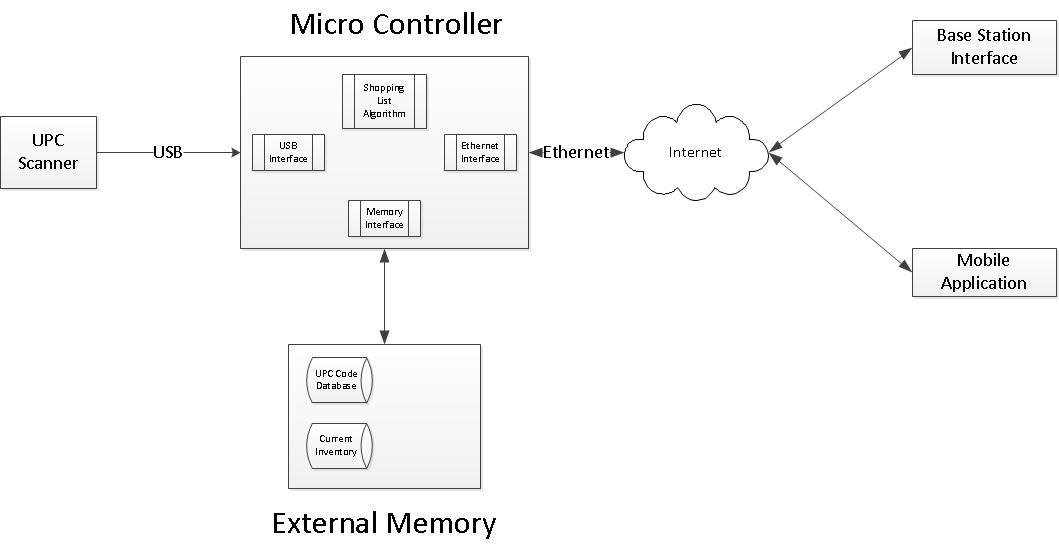
\includegraphics[scale=0.35]{SystemDiagram1}
\end{center}
\caption{High Level System Diagram}
\label{fig:sysdiag}
\end{figure}
\pagebreak
\section{Requirements Specification}
\subsection{Customer Needs}
\begin{enumerate}
\item The system should provide an intuitive, easy to use graphical interface.
\item The system should require minimal user input.
\item The system should be able to scan product codes.
\item The system should be able identify a scanned product code quickly.
\item The system should provide secure remote access.
\item The system should record product expiration dates.
\item The system should report items nearing expiration.
\item The system should provide access to the current inventory.
\item The system should provide a method to create and edit shopping lists.
\item The system should recommend shopping lists based on buying habits.
\item The system should function as an add-on to an existing refrigerator or pantry.
\end{enumerate}
\pagebreak
\subsection{Engineering Specifications}
\begin{table}[h!]
\begin{center}
\begin{tabular}{| p{1.2in} | p{2.5in} |p{2.5in} |}
\hline
Customer Need & Engineering Requirement & Justification \\
\hline
2,3,4 &A. An off-the-shelf UPC scanner should be used to input items. & A UPC scanner can read product codes with a single click.\\
\hline
4 &B. An internal UPC code database should be used to associate codes with items.&An internal database will remove delays associated with an internet look-up.\\
\hline
1,5,8&C. The system should be internet enabled and provide a web interface.&By providing a web interface any other internet-connected device can access the system.\\
\hline
5&D. Remote access should be authenticated with user name and password.&User names and passwords are standard for access control.\\
\hline
2,6&E. An internal database will store default recommended expiration estimates for common categories of items.&Inferring expiration dates based on item category helps minimizes user input. It is well known how long some products take to expire.\\
\hline
1,6&F. The user interface will provide a method for updating default expiration estimates.&Default estimates will not account for condition of product on arrival and may need to be updated.\\
\hline
1,7&G. Interface will provide a visual indication to the user when items are within a user-defined margin of expiration.&The goal of the system is to reduce waste due to expiration.\\
\hline
1,8&H. From both the base station and mobile application the user will be able to view an inventory list.&The user needs access to the current inventory in order to use items and shop effectively.\\
\hline
9,10&I. A database will be devoted to storing recommend shopping lists produced by the system.&User may wish to retain generic shopping lists for future use.\\
\hline
10&J. Recommended shopping lists will reflect purchasing history and expiration dates of current inventory.&Recommendation policy must suggest items relevant to the user in order to be useful.\\
\hline
9&K. Custom shopping lists, created either from the base station or the mobile interface, can be added to shopping list database.&Inefficient shopping practices can be prevented by storing shopping lists and the system can not anticipate all required items.\\
\hline
11&L. System will be self-contained and no modifications will be required to existing appliances.&Similar systems are commercially available but require costly replacement of existing appliances.\\
\hline
\end{tabular}
\end{center}
\end{table}
\section{Concept Selection}
\subsection{Evaluation of Existing Systems}
Many refrigerator systems are current available which offer integrated displays and internet connectivity. LG, Electrolux, and Samsung all offer refrigerators with large LCD displays that provide access to calendar applications, recipes, weather forecasts, and music and photo sharing services. The principle shortcoming of these devices is the elevated price and the need to completely replace existing appliances. As a more affordable alternative, tablet mounts are available for refrigerators as well.
However, these systems do not offer tracking of the refrigerator's contents and do not attempt to reduce waste or improve efficiency. LG demonstrated in April, 2011 a ``Smart Fridge" with goals closer to the proposed system. The sensors and algorithms used were not disclosed but the product objective is similar, tracking user purchases and providing a mobile interface to the refrigerator's contents while shopping \cite{lg}. Our system will provide a much more inexpensive alternative and will be more flexible; the system proposed will not be limited to strictly refrigerators and can be used as an add-on to an existing system.
\subsection{Concepts Considered and Chosen}
Many of the system design choices are easily derived from the engineering requirements; a UPC scanner with a standard USB interface is a clear choice for input of product codes and a mobile application is an obvious interface choice for a system catering to an on-the-go shopper. However, the choice of implementation platform and main base station display presents more alternatives. Expiration date recognition is also a potential shortcoming of the system; ideally image processing could be employed to read in expiration dates. However, the difficulty and computational complexity of applying image processing significantly extends the scope of the project and places additional performance constraints on the processing platform used. An evaluation of different expiration date recognition systems are tabulated in Table \ref{tab:datesys}, below.
\begin{table}[h!]
\begin{tabular}{| p{2in} | p{1in} | p{1.5in} | p{1.5in} | p{1.5in} |}
\cline{2-4}
\multicolumn{1}{c}{}&\multicolumn{3}{|c|}{Method} \\
\cline{2-4}
\multicolumn{1}{c|}{}&Entirely User Input&Predictive Strategy with User Override & Image to Text Recognition\\
\hline
Ease of Use&- - -&+&+ + +\\
\hline
Feasibility&+ + +&+ + +&-\\
\hline
Processing Power Required & + + + & + & - - -\\
\hline
Accuracy & + + + & - & + + +\\
\hline
\end{tabular}
\caption{Comparison of Expiration Date Systems}
\label{tab:datesys}
\end{table}
Ease of Use is one of the most critical system requirements, which eliminates a system relying completely on input from the user. However, feasibility and limiting processing performance required are important secondary objectives. Accuracy is critical to the goal of reducing waste due to expiration but there is inherently some variability even in reported expiration dates and image processing presents too much additional scope and too many additional requirements in exchange for marginal gains. As long as the predictive system learns from user input and anticipates that items will be purchased in different conditions, this scheme should be sufficient.
\newline \quad \newline
The choice of the base station main display and processing platform are linked but directed mainly by the processing platform. For example, if a personal computer was used a standard LCD monitor may be appropriate whereas if a tablet was chosen as the main processing engine the interface would be provided automatically. The most strongly considered option was to use a simple micro-controller to handle the processing load and to use a large, relative to the micro-controller, LCD display. Comparisons of different processing platform methods and different user interface choices for the base station are shown in Tables \ref{tab:proc} and \ref{tab:disp}, respectively.
\begin{table}[h!]
\begin{tabular}{| p{2in} | p{1in} | p{1.5in} | p{1.5in} | p{1.5in} |}
\cline{2-4}
\multicolumn{1}{c}{}&\multicolumn{3}{|c|}{Method} \\
\cline{2-4}
\multicolumn{1}{c|}{}&Personally Computer&Tablet (Combined UI and Processing)&Micro-controller\\
\hline
Processing Resources&+ + + &+ +&+\\
\hline
Cost &- - -& + &+ + +\\
\hline
Size&- - -&+ +&+ + +\\
\hline
\end{tabular}
\caption{Comparison of Main Processing Platforms}
\label{tab:proc}
\end{table}

\begin{table}[h!]
\begin{tabular}{| p{2in} | p{1in} | p{1.5in} | p{1.5in} | p{1.5in} |}
\cline{2-4}
\multicolumn{1}{c}{}&\multicolumn{3}{|c|}{Method} \\
\cline{2-4}
\multicolumn{1}{c|}{}&LCD PC Monitor&Tablet&LCD with Micro-controller\\
\hline
Integration with Unit&- - -&-&+ + +\\
\hline
Ease of Use&+ + +&+ + +&+\\
\hline
Size of Display& + + + &+ + +&+\\
\hline
GUI Quality&+ + +&+ + +&-\\
\hline
Size of Unit&- - -&+ + +&+ + +\\
\hline
\end{tabular}
\caption{Comparison of Main User Interface Displays}
\label{tab:disp}
\end{table}
\noindent Evaluating both the interface choice and the processing platform choice together eliminates the personal computer choice; a personal computer can not be integrated without significantly increasing the form factor of the system. A personal computer also greatly simplifies the system and strays away from an implementation tailored to this prototype. A tablet based interface was considered a very feasible alternative; however the cost and tailorability of the system are again concerns. A micro-controller based system is more appropriate for a small and specialized solution, with the principle concern being quality of the graphical interface produced compared with the other two methods. However, since the system will provide a general web interface, the mobile application as well as a variety of other possible interfaces can be used to view the display as well so the weight assigned to a high-quality base station interface is mitigated. Considering both choices together, the micro-controller route with an LCD display to visually inspect items as they are checked in and view inventory appears preferable.
\newline \quad \newline
Consideration of the these concerns, as well as the high level system diagram presented in Figure \ref{fig:sysdiag}, clarifies the separation of tasks while implementing the project. One group of tasks will contain the mobile interface and also development of an Interface Control Document (ICD) to enumerate the commands provided over the web interface. A second task group will consist of developing the internal databases, the expiration date warning system, and shopping list suggestion algorithm. The final group of tasks will consist of interfacing the micro-controller with the scanner, Ethernet interface, and with the main base station interface. The final task group will also contain development of the base station interface.



\begin{thebibliography}{9}
\bibitem{times}
\url{http://www.nytimes.com/2008/05/18/weekinreview/18martin.html?pagewanted=all}
\bibitem{lg}
\url{http://www.nytimes.com/2008/05/18/weekinreview/18martin.html?pagewanted=all}
 \end{thebibliography}

\end{document}